% This is samplepaper.tex, a sample chapter demonstrating the
% LLNCS macro package for Springer Computer Science proceedings;
% Version 2.20 of 2017/10/04
%
\documentclass[runningheads]{llncs}
%
\usepackage{amsmath}
\usepackage{amssymb}
\usepackage{booktabs} % For pretty tables
\usepackage{caption} % For caption spacing
\usepackage{subcaption}
\usepackage{graphicx}
\usepackage{pgfplots}
\usepackage[all]{nowidow}
\usepackage[utf8]{inputenc}
\usepackage{tikz}
\usetikzlibrary{er,positioning,bayesnet}
\usepackage{multicol}
\usepackage{algpseudocode,algorithm,algorithmicx}
\usepackage{hyperref}
\usepackage[inline]{enumitem} % Horizontal lists
\newcommand{\indentitem}{\setlength\itemindent{20pt}}

\graphicspath{{latex/}}
\newcommand{\card}[1]{\left\vert{#1}\right\vert}
\newcommand*\Let[2]{\State #1 $\gets$ #2}
\newcommand\qfrac[3][1pt]{\frac{%
		\ThisStyle{\addstackgap[#1]{\SavedStyle#2}}}{%
		\ThisStyle{\addstackgap[#1]{\SavedStyle#3}}%
}}


\newcommand{\F}{\ensuremath{\mathbb{F}}}
\newcommand{\B}{\ensuremath{\mathbb{B}}}
\newcommand{\LL}{\ensuremath{\mathbb{L}}}
\newcommand{\Me}{\ensuremath{\mathbb{M}_e^{\text{eff}}}}
\newcommand{\D}{\ensuremath{\text{D}}}
\renewcommand{\d}{\ensuremath{\text{d}}}
\pgfplotsset{compat=1.14}

\renewcommand{\topfraction}{0.85}
\renewcommand{\bottomfraction}{0.85}
\renewcommand{\textfraction}{0.15}
\renewcommand{\floatpagefraction}{0.8}
\renewcommand{\textfraction}{0.1}
\setlength{\floatsep}{3pt plus 1pt minus 1pt}
\setlength{\textfloatsep}{3pt plus 1pt minus 1pt}
\setlength{\intextsep}{3pt plus 1pt minus 1pt}
\setlength{\abovecaptionskip}{2pt plus 1pt minus 1pt}


\begin{document}
%
\title{A thermodynamically consistent multi-phase model of Extracellular Matrix}
%
\titlerunning{Mechanical Properties of ECM}
% If the paper title is too long for the running head, you can set
% an abbreviated paper title here
%
\author{Giulia Laura Celora}
%
%\authorrunning{F. Author et al.}
% First names are abbreviated in the running head.
% If there are more than two authors, 'et al.' is used.
%
\institute{Mathematical Institute University of Oxford}
%
\maketitle              % typeset the header of the contribution
%
\begin{abstract}

\end{abstract}
%
%
%
\section{Introduction}
There are now several studies supporting the central role of mechanical stimulus in tissue morphogenesis and homeostasis, alongside with biochemical signalling. \textit{In vitro} studies have shown that ECM rigidity and shear stresses can alone promote the transition to malignant phenotype of normal cells and consequently the growth of a tumour mass. Despite the well-known link between cell behaviour and mechanical stimuli, the lack of quantitative measurement has delayed our understanding of such phenomena. The development of new nanotechnology has now open to the possibility of measuring mechanical stresses by the use of external devices. Meanwhile, new techniques such as Atomic Force Microscopy (AFM) have been developed to measure the local mechanical properties of tissue, with atomic precision. Combining such information can boost our understanding and the development of a solid mathematical framework to describe tumour growth and exploit mechanics to improve and revolutionise current therapy against cancer. 

The aim of coupling micro-environment and cell behaviours requires a clear understanding of both and the investigation of phenomena occurring at different time and spacial scales. In this work we focus on the Extracellular Matrix (ECM), the external network of polymers supporting cells in tissues. Its mechanical properties, in particular its stiffness, contribute to determine the response of tissues to external mechanical stimuli. By controlling the composition of the matrix, its properties can be tuned to meet the function of a specific tissues. 

Experiments have shown that tumour development is associated to a stiffening of the tissue compared to the surrounding healthy one, despite the fact that tumour cells themselves are usually softer than normal ones. Such contradiction is just apparent, as ECM can account for such resistance to mechanical stimuli. As a result, cells are exposed to higher compressive stresses which can select for more aggressive and invasive phenotype of cancer cells, as well as favour the collapse of blood vessels and impede the diffusion of substances in the extra-cellular environment ultimately decreasing the efficacy of numerous therapies.

Usually approach to the modelling of solid tumour is the use of multi-phase theory, according to which tumour are equivalent to material consisting of a solid matrix of cells and ECM, and an interstitial fluid phase. Besides involving the use of fundamental laws such as conservation of mass and momentum, the formulation of the model requires the use of several constitutive equation for each of the phase considered. These dictate the macroscopic behaviour of the system and thus heavily affect the prediction of the model, and are usually based on experimental result and have thus a limited range of applicability. Having a more fundamental description of the system requires instead deriving such properties based on the microscopic behaviour of the system.   As mentioned before, there is little understanding on the properties of the fundamental components of the ECM.

\section{Non Equilibrium Thermodynamics.}
\label{secNET}
While equilibrium thermodynamics successfully apply to the description of ideal process, real processes are irreversible. In this cases, the change in entropy $\d S$ can result from the reversible exchange of energy and matter with the external environment, $\d_eS$ or the internal dissipation od energy during the process, $\d_iS$ \cite{NET}:
\begin{equation}
\d S = \d_eS + \d_iS, \hspace{5mm} \d_eS= \frac{\d Q}{T},
\end{equation}
where $Q$ is the amount of energy added to the environment and $T$ is the temperature. 
According to the second law of thermodynamics, which applies universally to any system or subsystem, $\d S_i\ge 0$.

For the purpose of this study, we will focus on isothermal process, i.e. $T=const$. Under this assumption, as derived by Gurtin in \cite{GURTIN}, the second law of thermodynamics is equivalent to the following \textit{energy imbalance inequality}:
\begin{equation}
\frac{\d}{\d t} \left\{\int_R \psi \right\}\leq W(R) + M(R) \label{energyin}
\end{equation}
where $R$ is a arbitrary control volume of the system, $\psi$ is the Helmholtz free energy, $W(R)$ is the rate at which the environment does work on $R$ and $M(R)$ is the inflow of mass due to transport. It is important to note that the energy inequality~(\ref{energyin}) holds for any isothermal process, independently of the specific physical system involved. Consequently, there is a constraint on the form the function $\psi$ can assume and how this can depend on the thermodynamic variables describing the system. 

The major focus of non-equilibrium thermodynamics is in defining the precise form of $\d_i S$, which, unlike $\d_e S$ is not a state function, but depends on the specific transformation applied to the system. 
Different theories have been proposed, \cite{NET}, each with its specific domain of applicability. In our study we will focus on \textquotedblleft Classical Irreversible Thermodynamics'' (CIT) which was pioneered by Onsager \cite{onsager} and Prigogine \cite{prigogine} in the first half of the 20th century. One of its most important assumptions is the \textit{Local Equilibrium Hypothesis}, which guarantees thermodynamic variables, including entropy, are locally well-defined, \cite{NET}. 
Consequently, we can introduce the entropy density $s=s(\mathbf{x},t)$ such that:
\begin{equation}
S = \int_{R} s \,\d V, \qquad \d s = \d_e s + \d_is, \qquad \d_is > 0, 
\end{equation}
and the local entropy production:
\begin{equation}
\sigma \equiv \frac{\d_i s}{\d t} \geq 0.
\end{equation}

Another central aspect of the theory is the introduction of \textit{thermodynamic forces} \footnote{Not to be intended in the mechanical sense} $F_m$ (causes) and \textit{thermodynamic fluxes} $J_m$ (effects) to describe the evolution of the irreversible transformation. These are related to $\sigma$ as follows:
\begin{equation}
\sigma = \sum_m F_m J_m.
\label{2law}
\end{equation}

While the local equilibrium hypothesis is at basis of most theories of non-equilibrium thermodynamics, the following two hypotheses are the one uniquely characterizing CIT:
\begin{itemize}
	\item[1.] \textit{Linear Relation between forces $F$ and fluxes $J$}:
	\begin{equation}
	J_m = \sum_k L_{mk} F_k,\label{lin}
	\end{equation}
	where the constant $L_{mk}$ are referred to as \textbf{phenomenological coefficients};
	\item[2.] \textit{Microscopic Reversibility}: time reversibility of processes at the micro-scale. 
\end{itemize}

Starting from two principles, in its seminal paper \cite{onsager} Onsager derives the well-known \textit{Onsager Reciprocal Relation}:
\begin{equation}
L_{mk}=L_{km}.
\end{equation}

If we now consider a isothermal transformation in the framework of CIT, alongside the energy imbalance inequality, the following equality must hold:

\begin{equation}
W(R)+M(R)-\frac{\d}{\d t} \left\{\int_R \psi \right\} = T \int_R \sigma \,\d V
\end{equation}

In the past few decades, CIT has been applied successfully to the modelling of several physical phenomena by engineers, physicists and applied mathematicians. However, this only applies to  phenomena near-equilibrium,for which a linear approximation of the flux-force relation holds. The growing interest in complex far-from-equilibrium phenomena has pushed toward the development of a more general framework to the study of non-equilibrium phenomena.  

\section{Extracellular Matrix.}
\label{ECMcomp}
Despite the tissue-specific nature of Extracellular Matrix (ECM), this is mainly composed of a network of collagen fibrils entangled with charged chains of glycosaminoglycans (GAGs). While collagen is mainly responsible for the mechanical behaviour of the tissue, GAGs can imbibe water, giving ECM the ability to swell while maintaining its structural integrity. As a result, the ECM behave as a polyelectrolyte gel \cite{ecm1,ecm2}. Besides being largely present in the natural world, synthetic polyelectrolytes are currently employed for a wide range of applications, such as drug delivery, biomedical devices, scaffolds for tissue engineering and soft robotics [ADD CITATIONS]. The increasing popularity of such material has boost the development of mathematical model of such systems, in particular focusing particularly on the their swelling and plastic behaviours [ADD CITATIONS].

\begin{figure}
	\begin{subfigure}{0.49\textwidth}
	\centering
	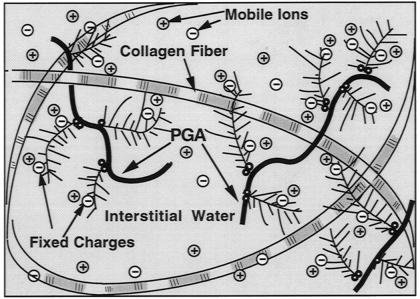
\includegraphics[scale=0.3]{images/ECM}
	\caption{}
	\end{subfigure}
	\begin{subfigure}{0.49\textwidth}
	\centering
	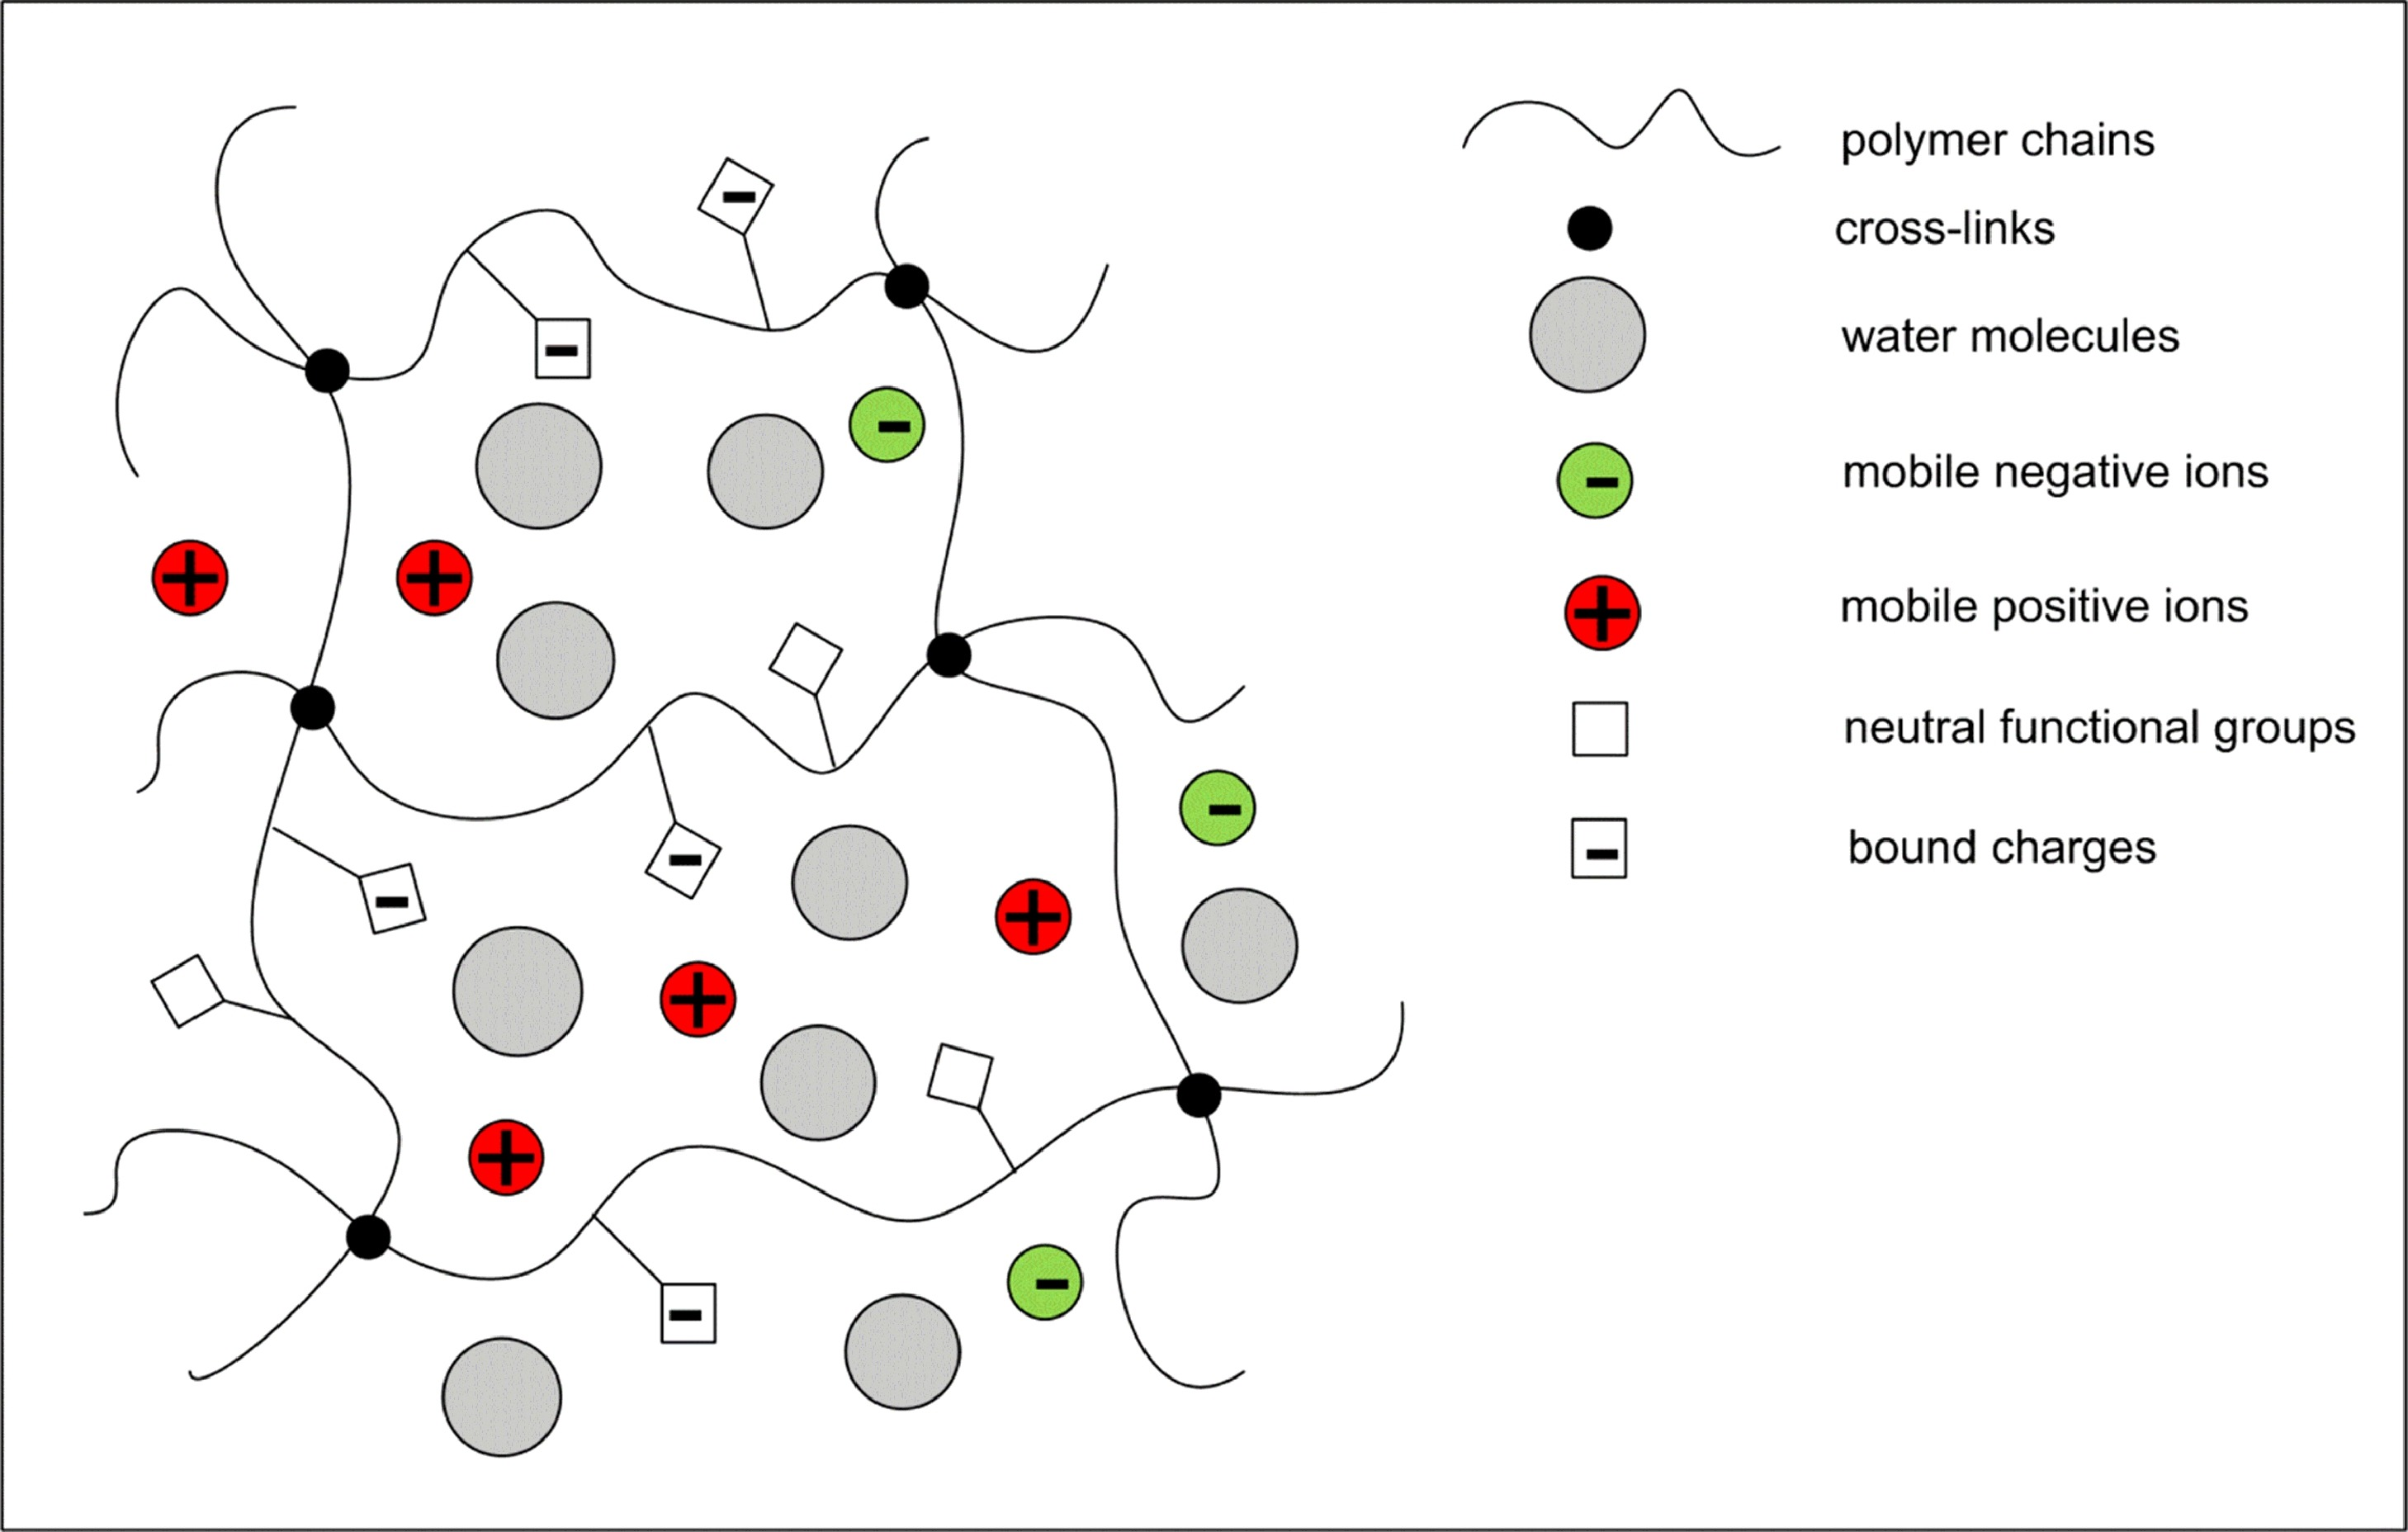
\includegraphics[scale=0.32]{images/ecmscheme.jpg}
	\caption{}
\end{subfigure}
\caption{Analogy between ECM in soft tissue and polyelectrolytes hydrogels: (a) schematic diagram of the structure of the charged hydrated articular cartilage, reproduced from \cite{pictureECM}; (b) an anionic polyelectrolyte gel modelled as a three-phase continuum, reproduced from \cite{DROZDOVph}.}
\end{figure}

There is now compelling evidence that the relaxation of stress in polymer gels, and thus in ECM is governed by the interplay of the poroelastic and viscoelastic nature of the gel. While the first determines the long range motion of solvents, visco-elastic dominates the stress relaxation dynamics at the microscopic level. Being the same level at which cells probe their environment, this suggests that the visco-elastic properties of the ECM might play a role in determining cell response [ADD ARTICLE IN NOTE AS CITATION].


\section{Model Development}
\subsection{Conservation Law.}

The ECM is here considered as a three-phase medium composed of a solid polymer network with fixed charges, a solvent (i.e. water molecules) and solutes (freely moving charges).

We here assume that the deformation of the ECM corresponds to the one of the solid network. As the tissue deform, the material element originally located at $\mathbf{X}$ in the initial configuration $\mathcal{B}_0$ is displaced to the point $\mathbf{x}$ in the current configuration $\mathcal{B}$. Such transformation is described by the deformation gradient $\F= \partial \mathbf{x}/\partial \mathbf{X}$, while the information about its change in the ECM volume due to swelling is encoded in $J= \det \F$. Since we assume the solid phase to be incompressible, any change in the volume can only be related to the migration of solvent and solutes molecules, whose nominal concentrations will be denoted by $C_s$ and $C_i$ respectively, $i=1,\ldots,N$ with $N$ number of free ion species. This lead to the molecular incompressibility condition:

\begin{equation}
 J= 1 + v_s C_s +\sum\limits_{i=1}^{N} v_i C_i
 \label{comp}
\end{equation}
where $v_m$ are the characteristic molecular volume of each species. As common in tissue modelling, we will here assume that the contribution of ions to the volume is negligible so that Equation~(\ref{comp}) reduces to:
\begin{equation}
J=1+v_s C_s.
\label{inc}
\end{equation} 

The volume fractions of fluid $\phi_f$ and solid $\phi_n$ phases in the gel are thus be defined as:
\begin{equation}
\phi_f = \frac{v_sC_s}{1+v_sC_s}, \qquad \phi_n = \frac{1}{1+v_sC_s}.
\end{equation}
where again we are neglecting the contribution of ions to the total volume.
While $C_m$ denote the number of each phase molecule per unit volume in the initial configuration, the actual concentration in the current state is denoted by $c_m=C_m/J$. Note that throughout this work we will be using $i=1,\ldots,N$ for denote only the concentration of ionic species, while $m\in\left\{s,1,\ldots,N\right\}$ to refer to both the solvent and solutes.

Mass conservation must apply to all mobile species and in the initial configuration these read:
\begin{equation}
\dot{C}_m + \nabla_0 \cdot \mathbf{J}_m = 0, 
\end{equation}
where $\mathbf{J}_m$ is the nominal flux per unit area in the dry state and $\nabla_0$ denote the gradient in the Lagrangian coordinate $\mathbf{X}$. Their counterparts in the actual configuration are denoted by $\mathbf{j}_m$ and $\nabla$ and are defined by the flow rule:
\begin{equation}
\mathbf{J}_m = J \F^{-1} \mathbf{j}_m, \qquad \nabla_0 (\cdot) = \F^{T} \nabla(\cdot).
\end{equation}

We also neglect any effect due to inertia, or any internal volume force so that the conservation of momentum for the gel reads:
\begin{gather}
\nabla_0 \cdot \mathbb{S}=0\\
\end{gather}
where $\mathbb{S}$ is the first Piola-Kirchoff tensor, which is related to the Cauchy stress tensor $\mathbb{T}$, as:
\begin{equation}
\mathbb{T} = J^{-1}\mathbb{S}\F^T.
\end{equation}

The presence of free moving ions generates and electric field which is denoted by $\mathbf{E}$ and $\mathbf{e}$ in the initial and current configuration respectively. Introducing the electrostatic potential $\Phi$, we have that:
\begin{equation}
\mathbf{E}= -\nabla_0 \, \Phi, \hspace{8mm} \mathbf{e}= - \nabla \, \Phi.
\end{equation}
As the gel is here considered to be a dielectric material, the presence of the field induces an electric displacement, which must satisfy Gauss law of electrostatics:
\begin{equation}
\nabla_0 \cdot \mathbf{H}= Q,
\label{gauss}
\end{equation}
where $\mathbf{H}$ is the nominal electric displacement and $Q$ is the local total charge, which accounts for both fixed and moving charges:
\begin{equation}
Q = e\left(\sum\limits_{i} z_i C_i+z_f C_{f}\right)\, , 
\end{equation}
where $e$ is the elementary charge, $C_f$ is the concentration of fix charges and $z_m$ is the valence of the corresponding charged species. Note that $C_f$ here corresponds to the concentration of GAGs, which is only a fraction of $C_s$. As for above, we can move from nominal quantities to the corresponding value in the current configuration by applying the following rules:

\begin{eqnarray}
\mathbf{H} = J \mathbf{h}\F^{-T},\\
\mathbf{E} = \F^T \mathbf{e},
\end{eqnarray}
where $\mathbf{h}$ is the electric displacement in the current configuration.

\subsection{Kinematics.}

As in [SARAH PAPER], we here consider that the initial state of the system $\mathcal{B}_0$ corresponds to the dry state of the gel. At any time $t$, the actual configuration of the body is $\mathcal{B}_t$. In this section, we want to focus on the rule according to which the body deforms from $\mathcal{B}_0$ to $\mathcal{B}_t$, which depends on the properties of the system studied. In our case, we consider a poro-visco-elastic material. As shown in Figure \ref{deformation}, there are two mechanisms that can contribute to the change in the body conformation: a volume preserving viscous deformation and long range transport of fluid that leads to swelling. 

\begin{figure}[h!]
	\centering
	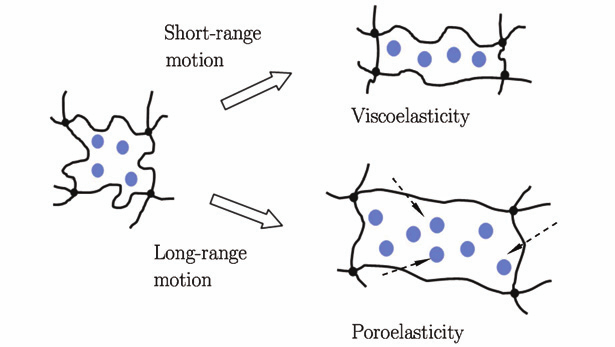
\includegraphics[scale=0.325]{images/visco_poro}
	\caption{Illustration of the molecular processes which account for a gel deformation: viscosity is related to change in the conformation of the network which results in short-range movement of fluid relative to the polymers; poro-elasticity is instead responsible for the long-range diffusion of solvent molecules in the gel/tissue. Reproduced from \cite{viscoporo}.}
	\label{deformation}
\end{figure}
 
We are here interested in the coupling of this two phenomena and how information from experiment at different spatial and temporal scale can be coupled. To do so, we will here present two different approaches that have been proposed in the literature to describe the complex mechanics of hydrogels. In particular, nanoscale rheological testing with AFM usually rely on a 1D \textit{Standard Linear Solid} model, as the one shown in Figure \ref{fig1}, to fit the experimental data \cite{Article1,viscoporo}.  

As pointed out by Hu et~al. \cite{viscoporo}, AFM measurements with nano-scale beads allow to capture the viscoelastic relaxation dynamics. But given the short length scale considered in the experiment, poroelastic relaxation is too fast to be captured. On the other hand, when considering larger time and spatial scale, such in standard compression test, the situation is reversed and what can be measure is the poroelastic dynamics. In this regime, the system can be well approximated by a poro-hyperelastic model \cite{Reviewpolyel,ecm2}. However, we are here interested in understanding how this two aspect interplay in determining the behaviour of the tissue. In the realm of soft matter, models have been proposed that either explicitly decouple the volumetric and isochoric deformation of the system \cite{magneto,NGUYEN}, see Figure \ref{figmode}(B1), or not \cite{Article1,CACCAVO2}, see Figure \ref{figmode}(A1). We here consider both constitutive models with the aim of comparing their predictions and identify any difference that would allow us to predict experimentally which of the two better describe the system under study. To avoid any confusion, we will denote them as model A and model B respectively. As an explanatory example of the non-equilibrium thermodynamics framework, we will here fully derive only the first model, see Figure \ref{figmode}(A1). The details on the derivation of the second model can instead be found in Appendix [Need to add the name]. 

\begin{figure}[h!]
	\hspace{-12mm}
	\begin{subfigure}{0.32\textwidth}
		\centering
		\large
	\def\svgwidth{0.95\linewidth}
	\input{latex/images/modelA1.pdf_tex}
	\caption*{\textbf{(A1)}}
	\label{fig1A}
	\end{subfigure}
	\begin{subfigure}{0.32\textwidth}
	\large
	\def\svgwidth{0.92\linewidth}
	\input{latex/images/modelB1.pdf_tex}
	\caption*{\textbf{(B1)}}
	\label{fig1B}
\end{subfigure}
\begin{subfigure}{0.34\textwidth}
	\Large
	\def\svgwidth{1.75\linewidth}
	\input{latex/images/modelA2.pdf_tex}
	\caption*{\textbf{(A2)}}
	\label{Model2}
\end{subfigure}
\vspace{5mm}
\caption{(A1) Rheological model for model A; (B1) rheological model for model B; (A3) multiplicative decomposition corresponding to model A.}
\label{figmode}
\end{figure}

Following a common approach in the large-deformation theory \cite{Article1,CACCAVO2,Plasto,magneto,NGUYEN,growthtum}, we base our derivation on a multiplicative decomposition of the deformation tensor $\F$, approach first proposed by Kr\"{o}ner in 1960 \cite{kro}:

\begin{equation}
\F=\F_e\F_v,\label{dec1}.
\end{equation}

As shown in Figure \ref{figmode}(A1), $\F_e$ is the elastic contribution to the deformation, with $J_e=\det \F_e>0$. On the other hand, the term $\F_v$ accounts for the viscous part of the deformation, which arise from the local rearrangement of molecules. As illustrate in Figure \ref{figmode}(A2), the multiplicative decomposition is equivalent to introducing an intermediate configuration $\mathcal{B}_v$, called natural or virtual configuration. Despite not being a real state of the system, it can be interpreted as the state the system would be in if it was instantaneously elastically unload. 

Using Equation~(\ref{dec1}), we can compute the velocity gradient tensor $\LL$:
\begin{equation}
\LL = \dot{\F}\F^{-1} = \LL_e + \F_e \LL_v \F_e^{-1},
\end{equation}
where $\LL_e=\dot{\F}_e\F_e^{-1}$ and $\dot{\F}_v\F_v^{-1}$ are respectively the elastic and viscous velocity gradient tensor. These can be decomposed in their symmetric and skewed part:

\begin{equation}
\begin{aligned}
\LL_e = \mathbb{D}_e + \mathbb{W}_e, \ \ \mathbb{D}_e = \frac{\LL_e+\LL^T_e}{2}, \ \ \mathbb{W}_e = \frac{\LL_e-\LL^T_e}{2};\\
\LL_v = \mathbb{D}_v + \mathbb{W}_v,  \ \ \mathbb{D}_v = \frac{\LL_v+\LL^T_v}{2}, \ \ \mathbb{W}_v = \frac{\LL_v-\LL^T_v}{2}.
\end{aligned}
\end{equation}

As mentioned before, the physical nature of the viscous deformation, molecular rearrangement, implies that $\F_v$ must preserve the volume, i.e. $J_v=\det \F_v= 1$. Despite agreeing with this argument, Caccavo et~al. \cite{Article1,CACCAVO2} do not include this constraint in their mathematical formulation. Consequently, our results will differ.

Despite the additional constraint, the decomposition~(\ref{dec1}) is not unique, as $\mathcal{B}_v$ would remained relaxed under any arbitrary rigid-body rotation \cite{multdec}. As suggested by \cite{Plasto}, in the case of isotropic material, it is reasonable to assume the viscous flow to be irrotational, i.e. $\mathbb{W}_v=\mathbb{O}$, so that $\LL_v \equiv \mathbb{D}_v$.
 
\subsection{Energy Balance Inequality.}
As mentioned in Section \ref{secNET}, the energy imbalance inequality impose restriction on the nature of the free energy $\psi$ of the system depending on how this exchanges energy and mass with the environment. Considering a control volume $R$ in the reference configuration, the system exchanges mass due to diffusion of each mobile species, so that $M(R)$ is given by:
\begin{equation}
M(R)= \sum\limits_{m=s,1,\ldots,N} - \int_{\partial R} \mu_m \,\mathbf{J}_m \cdot \mathbf{n} 
\end{equation}
where $\mathbf{n}$ is the unit normal vector to the surface $\partial R$ and $\mu_m$ is the chemical potential associated with each species. Widely used in the thermodynamics of mixture, the chemical potential is a measure of the rate of change in free energy associated with adding to a unit volume one more molecule. The work done on $R$ in the original configuration per unit time $W(R)$ is instead made up of two contributions, the electrical $W_{el}(R)$ and mechanical work $W_{mec}(R)$. Following \cite{DROZDOVph}, $W_{el}(R)$ is defined as:
\begin{equation}
W_{el}(R) = -\int_{\partial R} \Phi\, \dot{\mathbf{H}}\cdot \mathbf{n}
\end{equation}
As suggested by Gurtin \cite{GURTIN}, when accounting for the mechanical work, we consider also the effect of micro-stresses $\boldsymbol{\epsilon}$, which arise due to the system heterogeneity \cite{microstress}. As before we consider that the dominant contribution is related to the mixing of the solvent and solid phase, so that $W_{mec}(R)$ reads:
\begin{equation}
W_{mec}(R) = \int_{\partial R} \left(\boldsymbol{\xi}\cdot \mathbf{n}\right)\dot{C}_s + \int_{\partial R} \mathbb{S}\mathbf{n} \cdot \dot{\mathbf{u}}
\end{equation}
where $\mathbf{u}= \mathbf{x}-\mathbf{X}$ is the displacement vector, which is related to the deformation tensor, $\F=\mathbb{I}-\nabla_0 \mathbf{u}$. Substituting this result back into the energy imbalance, see Equation~(\ref{energyin}) and using the divergence theorem we obtain the following integral inequality:
\begin{equation}
\int_R \dot{\psi} - \mathbf{E}\cdot \dot{\mathbf{H}} \, + \, \sum\limits_{i=1}^{N} \left[e \Phi  z_i \dot{C}_i+ \nabla_0 \left(\mu_i \mathbf{J}_i \right)\right] + \nabla_0 (\mu_s \mathbf{J}_s- \boldsymbol{\xi}\dot{C}_s -\mathbb{S}^T\mathbf{\dot{u}}) \leq 0 
\end{equation}
Since the above inequality must hold for any choice of the volume $R$, the constraint must hold locally. So that:
\begin{equation}
\dot{\psi} - \mathbf{E}\cdot \dot{\mathbf{H}} \, + \, \sum\limits_{i=1}^{N} \left[e \Phi  z_i \dot{C}_i+ \nabla_0 \left(\mu_i \mathbf{J}_i \right)\right] + \nabla_0 (\mu_s \mathbf{J}_s- \boldsymbol{\xi}\dot{C}_s -\mathbb{S}^T\mathbf{\dot{u}}) \leq 0. 
\end{equation}
Further accounting for the balance laws presented in the previous section, we obtain that:
\begin{equation}
\begin{aligned}
\dot{\psi} - \mathbf{E}\cdot \dot{\mathbf{H}} \, + \, \sum\limits_{i=1}^{N} \left[e \Phi  z_i - \mu_i\right] \dot{C}_i - (\mu_s + \nabla_0 \cdot \boldsymbol{\xi})\,\dot{C}_s -\mathbb{S}:\dot{\F}\\
-\boldsymbol{\xi} \cdot \nabla_0 \, \dot{C}_s + \sum\limits_{m} \nabla_0 \, \mu_m \cdot \mathbf{J}_m \leq 0.
\end{aligned} 
\end{equation}

As exhaustively discussed in \cite{GURTIN,Plasto}, the energy imbalance inequality and the isotropic assumption on the system both impose restrictions on the constitutive equation for the free energy $\psi$. Adapting their results, to our specific problem, we have that:
\begin{equation}
\psi = \psi (\F,\F_e, C_s, C_i, \nabla C_s,\mathbf{H}).
\end{equation}

Based on this result, we can now assign the form of the function $\psi$, which will problem-dependent.
\subsection{Construction of the Free Energy.}
Following the standard approach in phase-field modeling, we assume that the total free energy is given by the superposition of each contribution. In our problem, there are six mechanisms that contributes to the energy: 

\begin{enumerate}
	{\indentitem\item[\textbullet] the energy of the electric field $\psi_1$;}
	{\indentitem \item[\textbullet] the energy of solvent and solutes' molecules not interacting with the solid phase $\psi_2$;}
	{\indentitem\item[\textbullet] the energy of mixing the solid phase with the solution, $\psi_3$;}
	{\indentitem\item[\textbullet] the energy of mixing the solvent with the solutes in solution, $\psi_4$;}
	{\indentitem\item[\textbullet] the interfacial energy between dissimilar phases, $\psi_5$;}
	{\indentitem\item[\textbullet] the energy of the solid phase not interacting with the solution, $\psi_6$.}
\end{enumerate}

Assuming the solid phase to be an ideal and linear dielectric material, with constant permittivity $\epsilon$,the free energy of polarization reads \cite{DROZDOV+,Reviewpolyel}:
\begin{gather}
\psi_1 = \frac{1}{2\epsilon J} \mathbf{H}\F^T \cdot \F \mathbf{H}.
\end{gather}

The specific energy density $\psi_2$ has the standard form:
\begin{equation}
\psi_1 = \sum\limits_{m} \mu^0_m C_m
\end{equation} 
where $\mu^0_m$ denote the chemical potential of non interacting solvent molecules and ions. Making use of the Flory-Huggins theory \cite{flory,hug}, the mixing energy is determined by the formula:
\begin{equation}
\psi_3 = \frac{k_B T J}{v_s} \left(\phi_f \ln \phi_f + \chi \phi_f \phi_n\right),
\end{equation}
where $k_B$ is the Boltzmann's constant, $T$ is the temperature and $\chi$ is the Flory-Huggins parameter, the adimensional parameter related to the enthalpy of mixing. It is worth mentioning also the approach of Xue et al. \cite{ecm1,ecm2}, where only the mixing of GAGs and solvent is assumed to contribute to the free energy. Despite GAGs having the main contribution on the swelling properties of the ECM, there is no direct experimental evidence that collagen not mixing with water. Moreover, in our model we are not explicitly differentiating between the two as separate entities, but as a unique network with fix charges, which coincide to the GAGs location.

When considering the contribution to the energy coming from the mixing of free ions with the solvent, it is commonly assumed that the solution is dilute \cite{Reviewpolyel,ecm1,ecm2}, so that $\psi_4$ reads:

\begin{equation}
\psi_4 = k_B T \sum\limits_{i=1}^{N} C_i \left(\ln \frac{C_i}{ C_s}-1\right).
\end{equation}

Differently from previous work on the modelling of soft tissue, we include the effect of interface tension, which is further couple to the mechanical deformation as proposed by Hong et al. \cite{Interface}. Note that as above, we assume that the contribution of ions in negligible, so that only the ideal solid-solvent interface plays a role:
\begin{equation}
\psi_5 = \frac{\gamma}{2} J \left|\nabla C_s\right|,
\end{equation}
where the constant $\gamma$ plays a role analogous to a surface tension.
Finally, we need to specify the mechanical energy density $\psi_6$, that without any loss of generality can be decomposed as:

\begin{equation}
\psi_6 = \psi_\mathbf{A}(\F) + \psi_\mathbf{B}(\F_e)
\end{equation}
where $\mathbf{A}$ and $\mathbf{B}$ refer to the branch of the standard linear solid model in Figure \ref{figmode} (A1) which is associated with the elastic energy.

As in \cite{ecm2}, we decide to model the collagen network as an isotropic and compressible Neo-Hookean material:

\begin{eqnarray}
\psi_\mathbf{A}(\F) = \frac{G_\mathbf{A}}{2} \left(\F:\F - 3 -2 \ln J\right)\\
\psi_\mathbf{B}(\F_e) = \frac{G_\mathbf{B}}{2} \left(\F_e:\F_e - 3 -2 \ln J_{e}\right)
\end{eqnarray}
where $G_\mathbf{\cdot}$ stands for the shear modulus associated with each branches, while $J$ and $J_e$ are as defined in the previous sections. The hyper-elastic nature of polymers network response can be derived in the realm of statical thermodynamics, assuming Gaussian chains and an affine network model \cite{floryprinciples}. However, other thermodynamically consistent stretching energy have been proposed in the literature, which can account based on other network models \cite{BERGSTROM1998931,boyce2,doi}.

\subsection{Entropy Production.}
\newpage
\bibliographystyle{splncs04}
\bibliography{latex/ref}
%
\end{document}
